%%%
%
% $Autor: Gautam Ramesh $
% $Date: 2025-10-31 11:15:45Z $
% $File: file.tex $
% $Version: 1 $
%
% ===========================================================================
% SECTION: APPLICATION DOMAIN KNOWLEDGE - SOFTWARE
% ===========================================================================
\chapter{Domain System - Software} \label{ch:domain_system_software}
\section{Application Domain Knowledge: Software}
\label{sec:software_domain}

While hardware provides the physical substrate for computational tasks, the software domain serves as the cognitive logic of the License Plate Recognition (LPR) system. In the context of embedded Edge AI, software architectures are defined not merely by application code, but by the rigid constraints of the underlying Operating System (OS) and the scarcity of physical resources.

This section details the software ecosystem, establishing the Operating System limitations, the engineered deployment pipelines, the memory management architecture (RAM vs. Swap), and the specific persistence logic used to store vehicle data and calculate parking duration.

% ---------------------------------------------------------------------------
% SUBSECTION: LEGACY ECOSYSTEM
% ---------------------------------------------------------------------------
\subsection{System Description: The Legacy Ecosystem}

A primary software constraint for this project is the NVIDIA JetPack SDK version supported by the Jetson Nano (4GB). Unlike modern desktop environments which update frequently, the Jetson Nano is locked to **JetPack 4.6**, which is built upon **Ubuntu 18.04 LTS**. This imposes a "Legacy Software Ecosystem" challenge.

\vspace{0.5cm}

% --- VISUAL 1: SOFTWARE STACK PYRAMID ---
\begin{figure}[htbp]
	\centering
		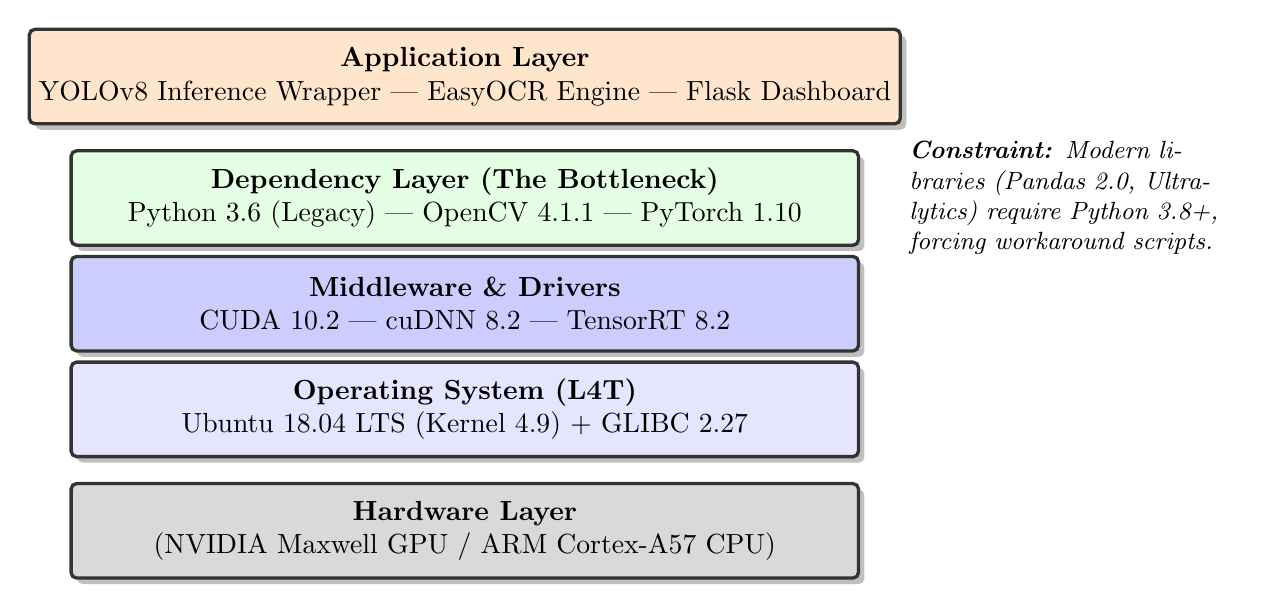
\begin{tikzpicture}[
		node distance=0cm,
		layer/.style={
			rectangle, 
			draw=black!80, 
			minimum width=10cm, 
			minimum height=1.2cm, 
			align=center, 
			very thick,
			rounded corners=2pt,
			drop shadow
		},
		arrow/.style={->, >=latex, very thick, gray}
		]
		
		% Stack from Bottom to Top
		\node[layer, fill=gray!30] (hw) {\textbf{Hardware Layer}\\(NVIDIA Maxwell GPU / ARM Cortex-A57 CPU)};
		
		\node[layer, fill=blue!10, above=0.3cm of hw] (kernel) {\textbf{Operating System (L4T)}\\Ubuntu 18.04 LTS (Kernel 4.9) + GLIBC 2.27};
		
		\node[layer, fill=blue!20, above=0.1cm of kernel] (drivers) {\textbf{Middleware \& Drivers}\\CUDA 10.2 | cuDNN 8.2 | TensorRT 8.2};
		
		\node[layer, fill=green!10, above=0.1cm of drivers] (deps) {\textbf{Dependency Layer (The Bottleneck)}\\Python 3.6 (Legacy) | OpenCV 4.1.1 | PyTorch 1.10};
		
		\node[layer, fill=orange!20, above=0.3cm of deps] (app) {\textbf{Application Layer}\\YOLOv8 Inference Wrapper | EasyOCR Engine | Flask Dashboard};
		
		% Annotations
		\node[right=0.5cm of deps, text width=4cm, font=\small\itshape, align=left] 
		{\textbf{Constraint:} Modern libraries (Pandas 2.0, Ultralytics) require Python 3.8+, forcing workaround scripts.};
		
	\end{tikzpicture}
	\caption{The Software Stack showing the dependency hierarchy and version locks.}
	\label{fig:software_stack}
\end{figure}

As visualized in Figure \ref{fig:software_stack}, this dependency layer creates a critical compatibility bottleneck. Modern AI libraries, such as \texttt{Ultralytics YOLOv8} and \texttt{Pandas 2.0}, natively require Python 3.8 or newer. The Jetson's default Python 3.6 environment is incompatible with these standard package distributions. 

To resolve this, we employed a **Custom Compilation Strategy**. Instead of installing pre-built binaries via \texttt{pip}, critical libraries (like \texttt{jetson-inference}) were compiled from source code directly on the device using \texttt{GCC 7.5.0}. This ensures that the application binaries are linked correctly against the legacy system libraries (glibc 2.27), preventing "ABI (Application Binary Interface) Incompatibility" errors during runtime.

% ---------------------------------------------------------------------------
% SUBSECTION: DEPLOYMENT PIPELINE
% ---------------------------------------------------------------------------
\subsection{Software Design and Installation Pipeline}

To overcome the computational limitations of the edge device, we adopted a \textbf{Split-Architecture Design}. Training a complex Convolutional Neural Network (CNN) directly on the Jetson Nano is unfeasible due to memory exhaustion and thermal throttling. Therefore, the "Installation" phase is not a single step but a pipeline spanning two distinct computing environments.

\vspace{0.5cm}

% --- VISUAL 2: DEPLOYMENT PIPELINE FLOWCHART ---
\begin{figure}[htbp]
	\centering
	
\usetikzlibrary{shapes, arrows.meta, positioning, fit, backgrounds, shadows, calc}

% --- DEFINING COLORS ---
\definecolor{hostblue}{RGB}{232, 241, 250}   % Light Blue background for PC
\definecolor{hostborder}{RGB}{70, 130, 180}  % Darker Blue for border
\definecolor{edgegreen}{RGB}{235, 250, 235}  % Light Green background for Jetson
\definecolor{edgeborder}{RGB}{34, 139, 34}   % Darker Green for border
\definecolor{nvidialime}{RGB}{118, 185, 0}   % NVIDIA Lime


	
	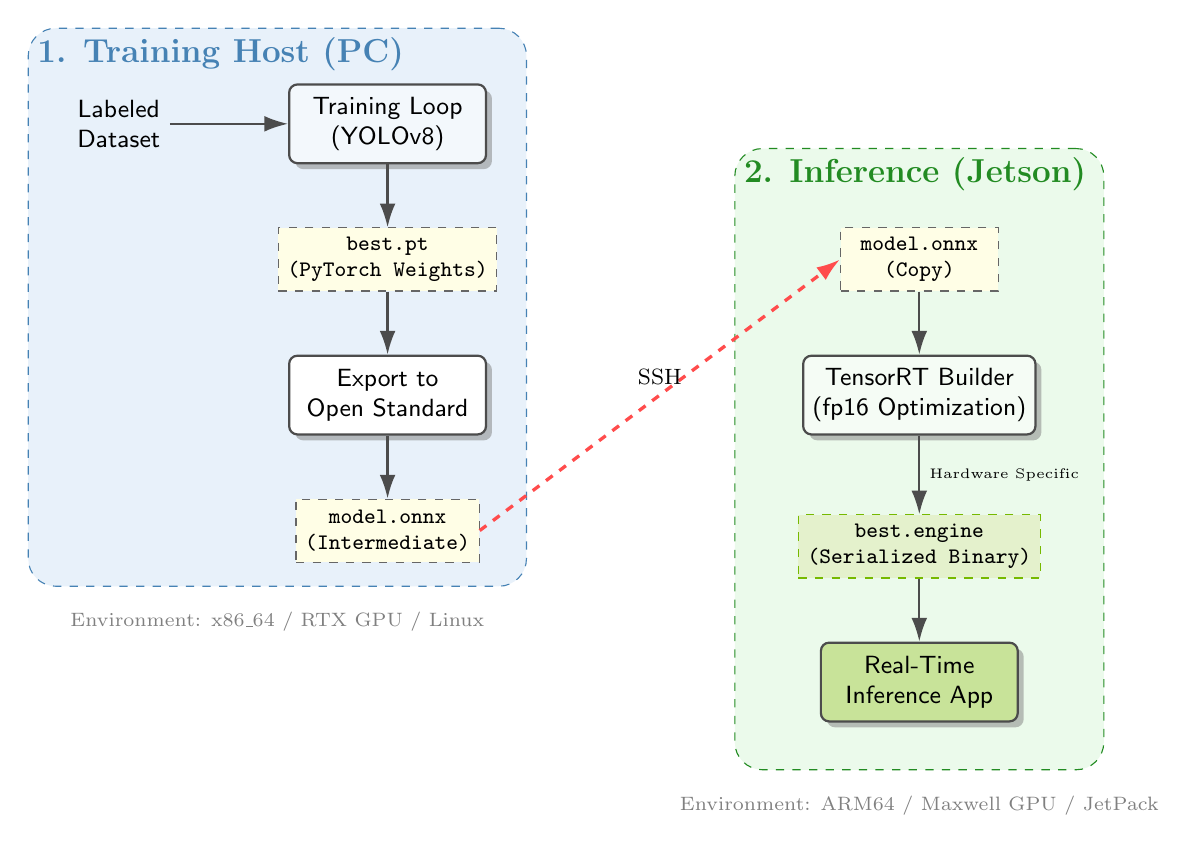
\begin{tikzpicture}[
		node distance=1.5cm and 1.5cm,
		font=\sffamily\small,
		% Node Styles
		process/.style={
			rectangle, 
			draw=black!70, 
			fill=white, 
			rounded corners=3pt, 
			minimum height=1cm, 
			minimum width=2.5cm, 
			align=center,
			drop shadow,
			thick
		},
		artifact/.style={
			rectangle, 
			draw=black!60, 
			fill=yellow!10, 
			dashed,
			minimum height=0.8cm, 
			minimum width=2cm, 
			align=center,
			font=\ttfamily\footnotesize
		},
		arrow/.style={
			-{Latex[length=3mm, width=2mm]}, 
			thick, 
			draw=black!70
		},
		labelbox/.style={
			font=\bfseries\large, 
			anchor=north west
		}
		]
		
		% --- ZONE 1: TRAINING HOST (Workstation) ---
		% Nodes
		\node[process, fill=hostblue!50] (training) {Training Loop\\(YOLOv8)};
		\node[artifact, below=0.8cm of training] (weights) {best.pt\\(PyTorch Weights)};
		\node[process, below=0.8cm of weights] (export) {Export to\\Open Standard};
		\node[artifact, below=0.8cm of export] (onnx) {model.onnx\\(Intermediate)};
		
		% Dataset Input
		\node[left=1.5cm of training, align=center] (dataset) {Labeled\\Dataset};
		\draw[arrow] (dataset) -- (training);
		
		% Internal Flows
		\draw[arrow] (training) -- (weights);
		\draw[arrow] (weights) -- (export);
		\draw[arrow] (export) -- (onnx);
		
		% --- ZONE 2: INFERENCE HOST (Jetson Nano) ---
		% We position this relative to the ONNX node to create a "bridge"
		\node[process, right=4cm of export, fill=edgegreen!50] (builder) {TensorRT Builder\\(fp16 Optimization)};
		
		% The "Transfer" logic
		\node[artifact, above=0.8cm of builder] (onnx_nano) {model.onnx\\(Copy)};
		\node[artifact, below=1cm of builder, fill=nvidialime!20, draw=nvidialime] (engine) {best.engine\\(Serialized Binary)};
		\node[process, below=0.8cm of engine, fill=nvidialime!40, thick] (inference) {Real-Time\\Inference App};
		
		% Internal Flows
		\draw[arrow] (onnx_nano) -- (builder);
		\draw[arrow] (builder) -- node[right, font=\tiny] {Hardware Specific} (engine);
		\draw[arrow] (engine) -- (inference);
		
		% --- CONNECTING THE WORLDS ---
		\draw[arrow, dashed, very thick, color=red!70] (onnx.east) -- node[above, font=\footnotesize, color=black] {SSH } (onnx_nano.west);
		
		% --- BACKGROUND BOXES ---
		\begin{scope}[on background layer]
			% Training Host Box
			\node[fit=(dataset)(training)(onnx)(export), 
			fill=hostblue, draw=hostborder, dashed, rounded corners=10pt,
			inner sep=0.5cm, yshift=0.2cm] (pc_box) {};
			\node[labelbox, text=hostborder] at (pc_box.north west) {1. Training Host (PC)};
			
			% Inference Host Box
			\node[fit=(onnx_nano)(builder)(inference)(engine), 
			fill=edgegreen, draw=edgeborder, dashed, rounded corners=10pt,
			inner sep=0.8cm, yshift=0.2cm] (nano_box) {};
			\node[labelbox, text=edgeborder] at (nano_box.north west) {2. Inference (Jetson)};
		\end{scope}
		
		% --- DECORATIVE HARDWARE SPECS (Optional text blocks) ---
		\node[below=0.2cm of pc_box, font=\scriptsize\color{gray}] {Environment: x86\_64 / RTX GPU / Linux};
		\node[below=0.2cm of nano_box, font=\scriptsize\color{gray}] {Environment: ARM64 / Maxwell GPU / JetPack};
		
	\end{tikzpicture}

	\caption{The Split-Architecture Deployment Pipeline used to bypass hardware limitations.}
	\label{fig:deployment_pipeline}
\end{figure}

The workflow illustrated in Figure \ref{fig:deployment_pipeline} addresses the "Cross-Compilation" challenge:
\begin{enumerate}
	\item \textbf{Training Host (PC):} The model is trained on a high-performance workstation using PyTorch. This environment handles the heavy matrix multiplications required for backpropagation.
	\item \textbf{Export (ONNX):} The model weights are exported to the Open Neural Network Exchange (ONNX) format (Opset 11). This step strips away Python-specific dependencies, leaving only the computational graph.
	\item \textbf{Inference Host (Jetson):} The ONNX file is transferred to the Jetson, where it is compiled into a \textbf{TensorRT Engine} plan. This binary format is optimized for the Nano's Maxwell GPU architecture, utilizing \textbf{FP16 (Half-Precision)} arithmetic. This optimization reduces the memory bandwidth requirement by 50\%, yielding a 40--50\% improvement in inference speed compared to raw PyTorch execution.
\end{enumerate}

% ---------------------------------------------------------------------------
% SUBSECTION: MEMORY MANAGEMENT (RAM)
% ---------------------------------------------------------------------------
\subsection{Memory Management Architecture}

A defining characteristic of the embedded software domain is the scarcity of Random Access Memory (RAM). The Jetson Nano possesses a \textbf{Unified Memory Architecture} where the CPU and GPU share a single 4GB physical pool. This creates a "Zero-Sum Game": every megabyte used by the Ubuntu OS is a megabyte denied to the AI model.

During stress testing, the simultaneous load of the OS ($\approx 1.2$ GB), the Object Detector ($\approx 1.5$ GB), and the OCR Engine ($\approx 1.0$ GB) resulted in a total demand exceeding 4GB. This triggered the Linux kernel's \textbf{OOM (Out of Memory) Killer}, which terminates processes to prevent a system crash.

\vspace{0.5cm}

% --- VISUAL 3: MEMORY MAP DIAGRAM ---
\begin{figure}[htbp]
	\centering
		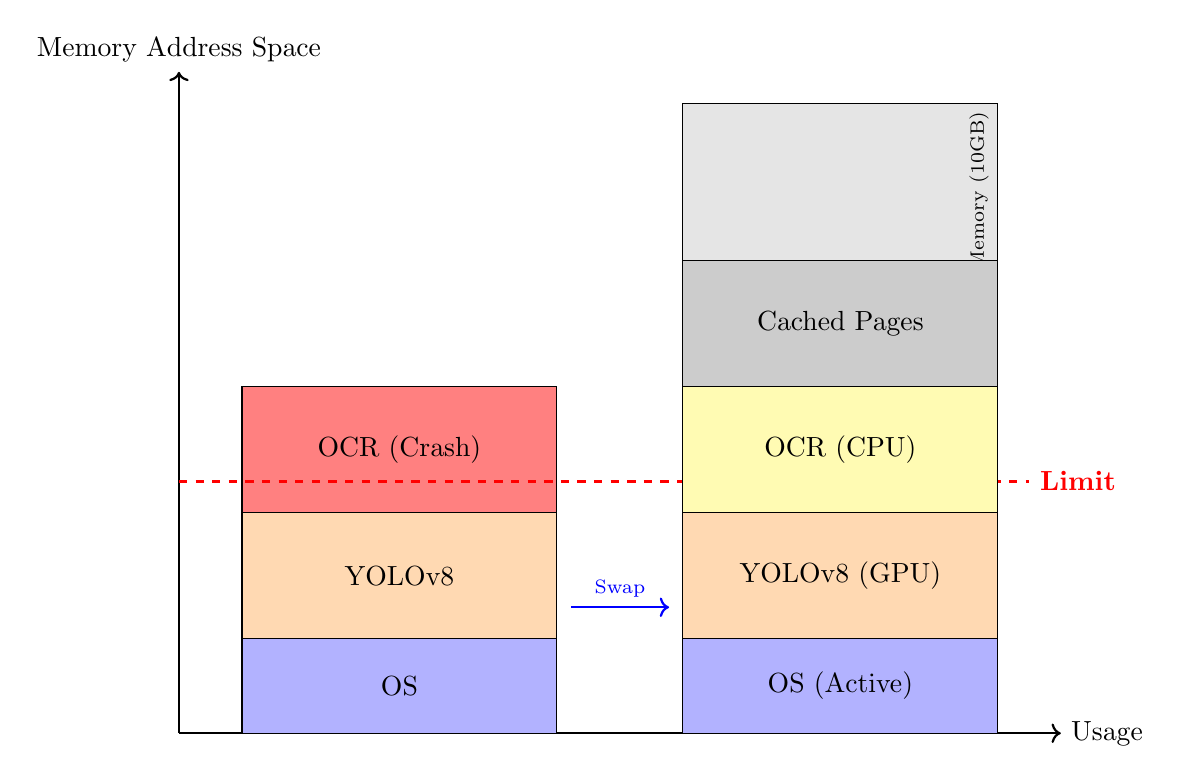
\begin{tikzpicture}[scale=0.8]
		% Axes - Extended to cover the extra width (up to x=14)
		\draw[thick, ->] (0,0) -- (0,10.5) node[above] {Memory Address Space};
		\draw[thick, ->] (0,0) -- (14,0) node[right] {Usage};
		
		% --- LEFT COLUMN: PHYSICAL RAM (Width = 5 units) ---
		% Range: x=1 to x=6 (Center x=3.5)
		
		% The Container Bar
		\draw[fill=green!20] (1,0) rectangle (6,4);
		% Label rotated to fit vertically along the side
		\node[rotate=90] at (5.7, 2) {\scriptsize Physical RAM (4GB)};
		
		% Stack Items (Centered at x=3.5)
		\draw[fill=blue!30] (1,0) rectangle (6,1.5);   \node at (3.5,0.75) {OS};
		\draw[fill=orange!30] (1,1.5) rectangle (6,3.5); \node at (3.5,2.5) {YOLOv8};
		\draw[fill=red!50] (1,3.5) rectangle (6,5.5);    \node at (3.5,4.5) {OCR (Crash)};
		
		% OOM Threshold Line (Extended)
		\draw[red, very thick, dashed] (0,4) -- (13.5,4) node[right, red, font=\bfseries] {Limit};
		
		% --- RIGHT COLUMN: VIRTUAL MEMORY (Width = 5 units) ---
		% Range: x=8 to x=13 (Center x=10.5)
		
		% The Container Bar
		\draw[fill=gray!20] (8,0) rectangle (13,10);
		\node[rotate=90] at (12.7, 8) {\scriptsize Virtual Memory (10GB)};
		
		% Stack Items (Centered at x=10.5)
		\draw[fill=blue!30] (8,0) rectangle (13,1.5);   \node at (10.5,0.75) {OS (Active)};
		\draw[fill=orange!30] (8,1.5) rectangle (13,3.5); \node at (10.5,2.5) {YOLOv8 (GPU)};
		\draw[fill=yellow!30] (8,3.5) rectangle (13,5.5); \node at (10.5,4.5) {OCR (CPU)};
		\draw[fill=gray!40] (8,5.5) rectangle (13,7.5);   \node at (10.5,6.5) {Cached Pages};
		
		% Arrow connecting the two columns
		\draw[->, thick, blue, shorten >= 5pt, shorten <= 5pt] (6, 2) -- (8, 2) node[midway, above, font=\scriptsize] {Swap};
		
	\end{tikzpicture}
	\caption{Memory Allocation Strategy: Expanding physical limits with SSD Swap.}
	\label{fig:memory_architecture}
\end{figure}

To resolve this, we engineered a virtual memory expansion using a \textbf{6GB Swap Partition} on the external SSD (Figure \ref{fig:memory_architecture}). This strategy allows the OS to "page out" inactive memory blocks (such as the Desktop GUI and background services) to the SSD, reserving the high-speed physical RAM for the active CUDA tensors required by the AI inference engine. By placing the Swap on a high-speed SSD (USB 3.0) rather than the slower SD card, we minimize the latency penalty known as "Swap Thrashing."

% ---------------------------------------------------------------------------
% SUBSECTION: DATA STORAGE & LOGIC (SQLITE)
% ---------------------------------------------------------------------------
\subsection{Data Persistence and Business Logic}

Reliable data storage is critical for an automated parking system. Unlike volatile memory (RAM), the system requires a persistent storage layer to ensure that parking records are preserved during power cycles or system reboots.

\subsubsection{Storage Offloading Strategy}
The Jetson Nano boots from a microSD card, which is inherently prone to corruption if subjected to heavy write cycles (e.g., continuous database logging). To mitigate this risk, we implemented a \textbf{Storage Offloading} architecture:
\begin{itemize}
	\item \textbf{Internal Storage (SD Card):} Reserved strictly for the Read-Only Operating System and system libraries.
	\item \textbf{External Storage (SSD):} The application database (\texttt{parking.db}) and logs are physically stored on the mounted SSD partition at \texttt{/media/myssd}. This drive utilizes the **EXT4** journaling file system, providing superior data integrity against power loss.
\end{itemize}

\subsubsection{Database Schema (SQLite)}
We utilized \textbf{SQLite}, a serverless, self-contained SQL database engine, rather than a client-server database like MySQL. This reduces memory overhead while providing full ACID (Atomicity, Consistency, Isolation, Durability) compliance. The data is structured in a single normalized table:

\begin{itemize}
	\item \textbf{Table Name:} \texttt{visits}
	\item \textbf{Column 1:} \texttt{plate} (TEXT, Primary Key) - The unique license plate identifier.
	\item \textbf{Column 2:} \texttt{entry\_ts} (REAL) - The Unix timestamp of the first detection event.
	\item \textbf{Column 3:} \texttt{last\_seen\_ts} (REAL) - The Unix timestamp of the most recent detection.
\end{itemize}

\subsubsection{Car Park Duration Algorithm}
The core business logic—calculating the parking duration and fee—is derived dynamically from the timestamps. The system uses a "State-Based" calculation rather than an incrementing counter. This stateless design ensures accuracy even if the software restarts or crashes mid-session.

The duration $\Delta t$ is calculated as:
\begin{equation}
	\Delta t = t_{current} - t_{entry\_ts}
\end{equation}

Where $t_{current}$ is the system time at the moment of the request. The parking fee ($C$) is then derived by applying the billing rate ($R$):
\begin{equation}
	C = \Delta t \times R \quad (\text{e.g., } R = 0.10 \text{\euro}/s)
\end{equation}

This approach ensures that the financial calculation is deterministic and historically reconstructible. The system utilizes **Python Threading** to handle video processing and database I/O concurrently, ensuring that database writes do not block the video feed frame rate.

% ---------------------------------------------------------------------------
% SUBSECTION: REMOTE PROTOCOLS
% ---------------------------------------------------------------------------
\subsection{Protocols and Remote Development Strategy}

An important milestone was solving challenges regarding standard development tools. The VS Code Remote Server requires \texttt{glibc 2.28}, whereas the Jetson's OS is locked to \texttt{glibc 2.27}. This incompatibility rendered standard remote debugging impossible.

To circumvent this, we architected a protocol switch from the standard VS Code Server agent to a lightweight \textbf{SSH-FS (Secure Shell File System)} implementation.

\vspace{0.5cm}

% --- VISUAL 4: REMOTE PROTOCOL DIAGRAM ---
\begin{figure}[htbp]
	\centering
		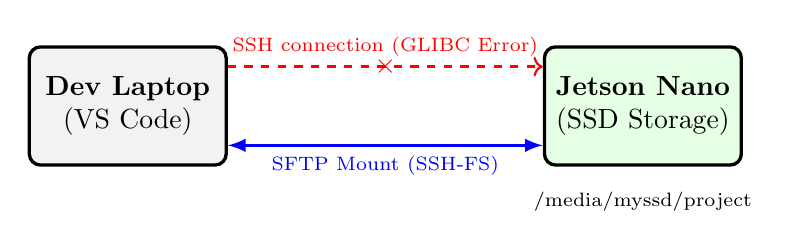
\begin{tikzpicture}[
		node distance=3cm,
		device/.style={
			rectangle, 
			draw=black, 
			very thick, 
			minimum width=2.5cm, 
			minimum height=1.5cm, 
			align=center, 
			rounded corners
		},
		connection/.style={
			<->, 
			>=latex, 
			very thick, 
			blue
		}
		]
		
		\node[device, fill=gray!10] (laptop) {\textbf{Dev Laptop}\\(VS Code)};
		\node[device, fill=green!10, right=4cm of laptop] (jetson) {\textbf{Jetson Nano}\\(SSD Storage)};
		
		% Failed Connection
		\draw[->, thick, red, dashed] ($(laptop.east)+(0,0.5)$) -- node[midway, above, font=\scriptsize, red] {SSH connection (GLIBC Error)} ($(jetson.west)+(0,0.5)$);
		\node[red] at ($(laptop.east)!0.5!(jetson.west)+(0,0.5)$) {$\times$};
		
		% Success Connection
		\draw[connection] ($(laptop.east)+(0,-0.5)$) -- node[midway, below, font=\scriptsize, blue] {SFTP Mount (SSH-FS)} ($(jetson.west)+(0,-0.5)$);
		
		% Label
		\node[below=0.2cm of jetson, font=\scriptsize] {/media/myssd/project};
		
	\end{tikzpicture}
	\caption{Remote Development Protocol: Switching from Binary Agents to File System Mounting.}
	\label{fig:remote_protocol}
\end{figure}

As depicted in Figure \ref{fig:remote_protocol}, instead of running a binary agent on the Jetson, we mount the Jetson's filesystem locally on the development laptop via the SSH protocol (Port 22). This allows code editing using the laptop's modern environment while files are physically saved to the Jetson's SSD in real-time. This eliminates the need for heavyweight server-side dependencies on the edge device.